\begin{exercise}{Système optomécanique}{3}{Spé}
{Interférences, pression de radiation, Fabry-Pérot}{lelay}

On considère le système optomécanique réprésenté ci-dessous : la lumière est introduite dans le système par la gauche dans une cavité de section transverse $S$ formée par deux miroirs. Le miroir de gauche est immobile et parfaitement réfléchissant, le miroir de droite est mobile, a un coefficient de réflexion $r$ très proche de 1, possède une masse $m$ très faible et est relié au fond de la cavité par un ressort de raideur $k$.

\begin{center}
    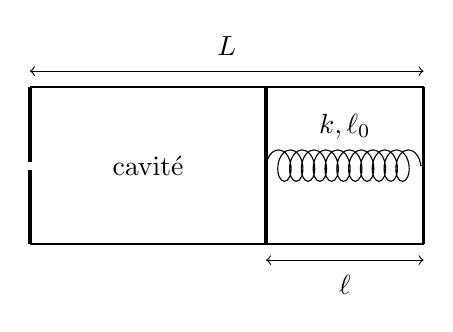
\begin{tikzpicture}
    \draw[<->] (-1,1.2) -- (4, 1.2);
    \draw (1.5,1.2) node[above=2pt] {$L$};
    
    % \fill[black!5]  (0,-1) rectangle (2,1);
    \draw[ultra thick] (-1,-1) -- (-1, -0.05);
    \draw[ultra thick] (-1,0.05) -- (-1, 1);
    \draw[thick] (-1,-1) -- (4,-1);
    \draw[thick] (-1, 1) -- (4, 1);
    \draw[ultra thick] (2,-1) -- (2, 1);
    \draw (0.5,0) node[anchor=center] {cavité};
    
    \draw[decoration={aspect=0.6, segment length=1.5mm, amplitude=2mm,coil},decorate] (2,0) -- (4,0);
    \draw[thick] (4,-1) -- (4, 1);
    \draw (3,0) node[above=6pt] {$k, \ell_0$};

    \draw[<->] (2,-1.2) -- (4, -1.2);
    \draw (3,-1.2) node[below=2pt] {$\ell$};
    
    \end{tikzpicture}
\end{center}

\begin{questions}
    \questioncours Phénomène d'interférences
    \question Calculer $I$, l'intensité lumineuse sur le miroir.
    \uplevel{La lumière est composée de photons, d'énergie $h\nu$ et de quantité de mouvement $h/\lambda$ (relation de De Broglie). On note $n$ la densité volumique de photons en un point.}
    \question En assimilant l'énergie du champ électromagnétique à celle des photons, donner un lien entre $n$ et $I$.
    \question En déduire, à l'aide d'un bilan de quantité de mouvement sur un temps $\dd{t}$, la force de pression de radiation qu'une onde lumineuse d'intensité $I$ exerce lorsqu'elle est réfléchie sur un miroir perpendiculaire à sa direction de propagation
    \question Donner les positions d'équilibre du miroir mobile et de leur stabilité.
\end{questions}
\end{exercise}

\begin{solution}

\begin{questions}
    \questioncours Phénomène d'interférences
    \question C'est un fabry-Pérot. Entre deux aller-retours, la différence de marche est $\delta = 2(L-\ell)$ d'où un déphasage $\Phi = 2\pi \delta/\lambda = 4\pi(L-\ell)/\lambda$ et l'amplitude est divisée par $r$, on trouve 
    \begin{align}
        A = A_0 + r A_o e^{i\Phi} + \cdots= \frac{A_0}{1 - re^{i\Phi}}
    \end{align}
    d'où l'intensité 
    \begin{align}
        I &= |A|^2 = \frac{I_0}{1 + r^2 - 2r\cos\Phi} \\
        &= \frac{I_0}{(1-r)^2} \frac{1}{1 + \cal{F}\sin^2(\Phi/2)}
    \end{align}
    sous la forme de la fonction d'Airy, avec la finesse standard $\cal{F} = 4r/(1-r)^2$.
    
    FAIRE TRACER LA COURBE AUX ETUDIANTS

    Puisque $r$ est proche de 1, on prendra la finesse très grande et donc les franes brillantes sont très piquées.
    \uplevel{La lumière est composée de photons, d'énergie $h\nu$ et de quantité de mouvement $h/\lambda$ (relation de De Broglie). On note $n$ la densité volumique de photons en un point.}
    \question Densité d'energie EM $\frac12 \epsilon_0 E^2$, intensité lumineuse $I = E^2$, densité d'énergie photonique $n h \nu$ d'où $n h \nu = \frac12 \epsilon_0 I$ et donc $n =\epsilon_0 I/(2 h \nu)$
    \question Pendant $\dd{t}$ le miroir réfléchit $n (c\dd{t}) S$ photons de qté de mvt $h/\lambda$ d'où $\dd{p} = n c S \dd{t} \cdot 2 \cdot h/\lambda = 2 n h \nu S \dd{t} =\epsilon_0 I S \dd{t}$ et donc la force de pression de radiation $P = \epsilon_0 I$.
    \question Résolution graphique : Tracer $P(\ell)$ (successions de pics fins) et la force du ressort $F(\ell)$ (droite décroissante), voir où sont les intersections. Discuter le cas d'une raideur très grande, très petite. À chaque intersection de la droite avec un pic il y a une position stable et une instable (je crois). On peut calculer la freq des petites oscillations en faisant un DL ? Discuter en tout cas les pertes, qui n'ont pas été abordées ici.
\end{questions}
\end{solution}